\section{Mathematical Concept}

\begin{frame}
    \frametitle{Mathematical Explanation}
    Let $D = \{(x_{1},y_{1}), (x_{2}, y_{2}), ... , (x_{N}, y_{N})\}$ 
    and $T_{D,\theta}$ is fully grown decision tree trained on set $D$ with using parameters $\theta$.
    Random Forest estimate of an observation $x^*$ is
    \begin{block}{Majority Voting}
        \begin{equation}
            \boldsymbol{RF}_{D, \theta_{1}, \theta_{2}, ..., \theta_{B}} (x^*) =
            \underset{c \in Y}{argmax} \sum_{b = 1}^{B}{1(\hat{T}_{b}(x^*) = c)}
        \end{equation}
    \end{block}
    \begin{block}{Soft Voting}
        \begin{equation}
            \boldsymbol{RF}_{D, \theta_{1}, \theta_{2}, ..., \theta_{B}} (x^*) =
            \underset{c \in Y}{argmax} \dfrac{1}{B}\sum_{b = 1}^{B}{\hat{p}_{D, \theta_{b}} (Y = c | X = x^*)}
        \end{equation}
    \end{block}
    where $\hat{p}_{D, \theta_{b}} (Y = c | X = x^*)$ is the probability estimates of a tree.
\end{frame}
\begin{frame}
    \frametitle{Majority Voting}
    \begin{figure}
        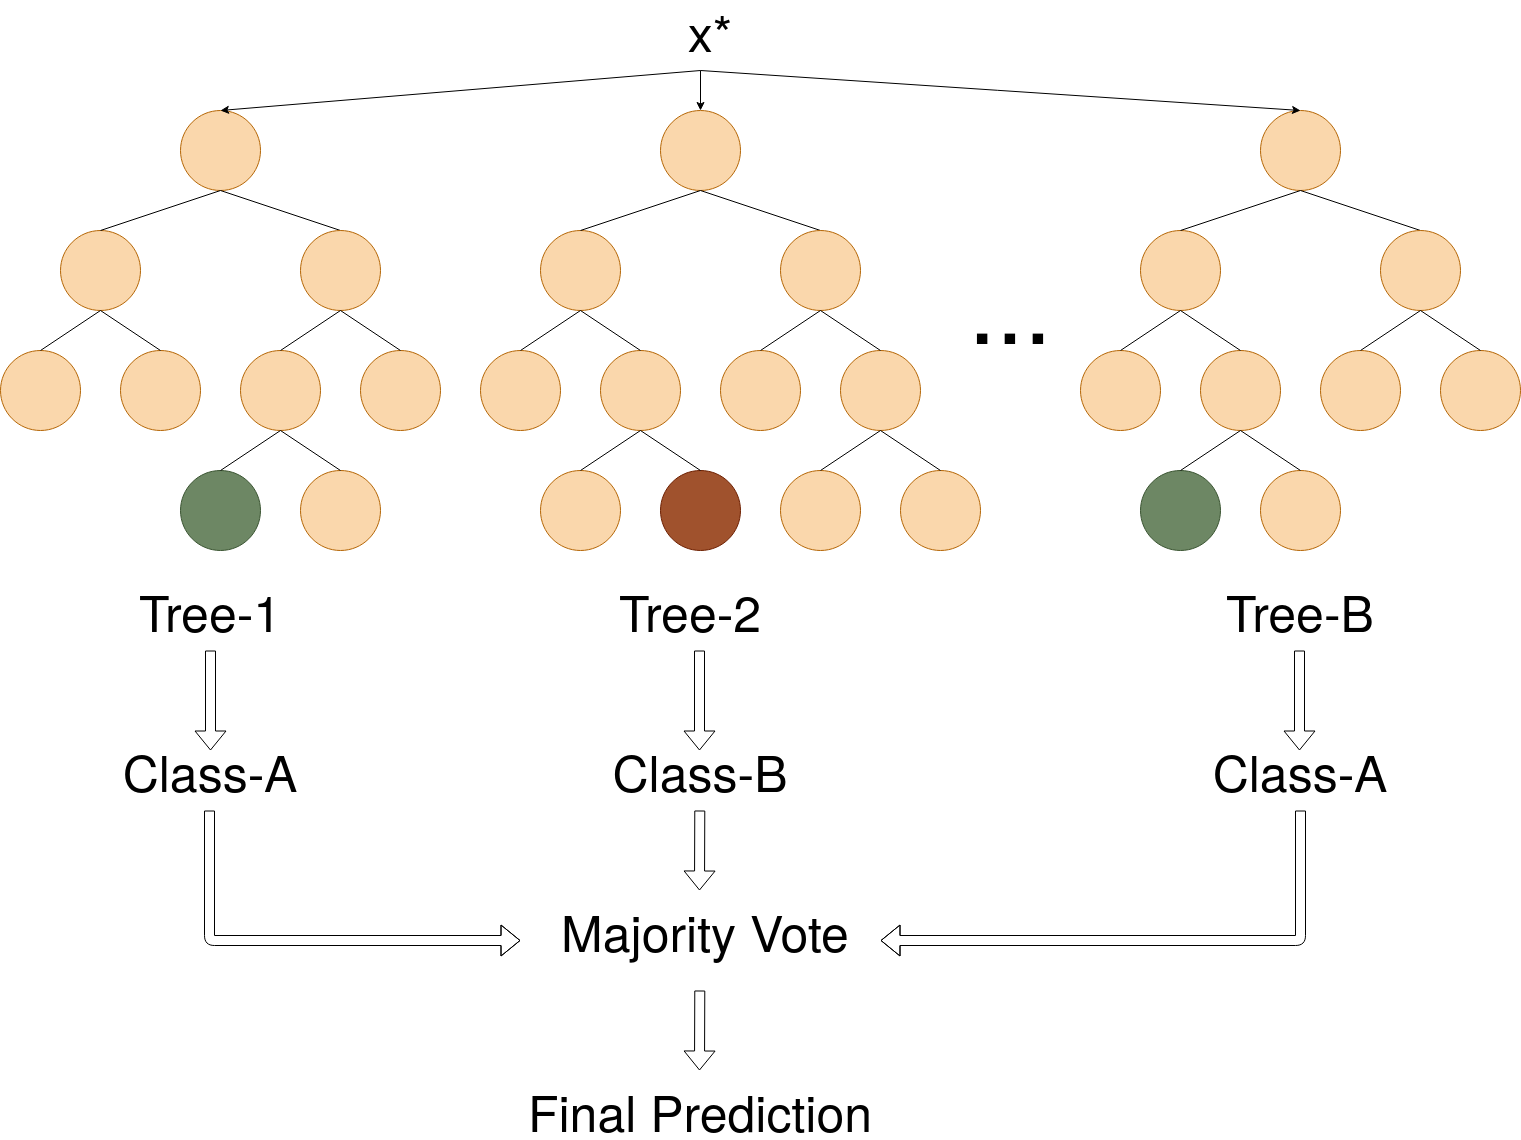
\includegraphics[height=0.7\textheight]{images/majority.png}
        \caption{Majority Voting Illustration}
    \end{figure}
\end{frame}
\begin{frame}
    \frametitle{Soft Voting}
    \begin{figure}
    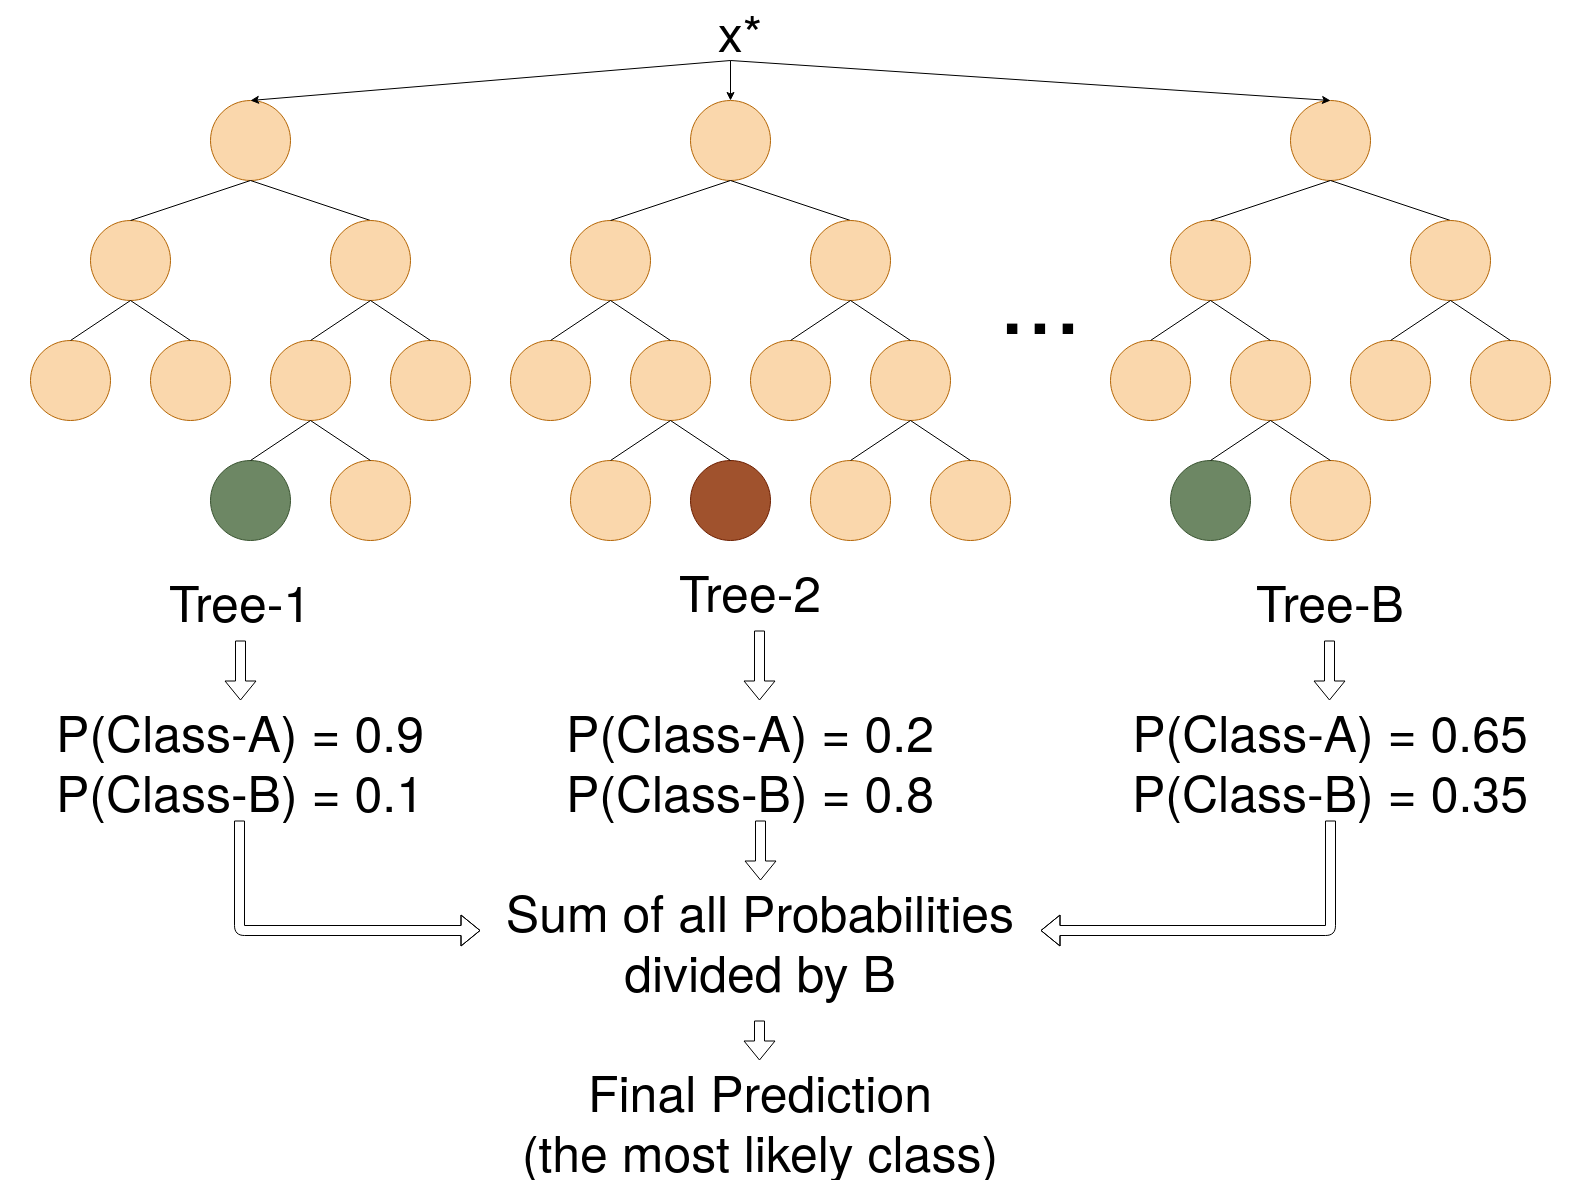
\includegraphics[height=0.7\textheight]{images/soft.png}
    \caption{Soft Voting Illustration}
    \end{figure}
\end{frame}
\begin{frame}
    \frametitle{Bayes Model}
    Theoretically, there exists a model that minimizes the generalization error and can be derived analitically independent of the model \cite{louppe2014understanding}.
    Conditioning the expected generalization error on X gives:
    \begin{equation}
        \mathbb{E}_{X,Y} \{L(Y, \phi_{\beta}(X))\} = \mathbb{E}_{X}\{\mathbb{E}_{Y|X}\{L(Y, \phi_{\beta}(X)) \} \}
    \end{equation}
    Point-wise minimization of inner term yields:
    \begin{equation}
        \phi_{\beta} = \underset{c \in Y}{argmin} \; \mathbb{E}_{Y|X=x}\{L(Y,c)\}
    \end{equation}
    $\phi_{\beta}$ is Bayes Model and as mentioned $\boldsymbol{Err}(\phi_{\beta})$ is the irreducible error.
\end{frame}
\begin{frame}
    \frametitle{The Expected Generalization Error}
        The expected generalization error of $T_{D,\theta}$ is
        \begin{equation}\label{eq:exp_gen_error}
            \boldsymbol{Err}(T_{D,\theta}) = \mathbb{E}_{X,Y}\{L(Y, T_{D,\theta}(X)) \}
        \end{equation}
        with the decomposition as
        \begin{equation}
        \boldsymbol{Err}(T_{D,\theta}) = noise(x) + bias^2(x) + var(x)
    \end{equation}
    \qquad \quad where
    \begin{align}
        & noise(x) = \boldsymbol{Err}(\phi_{\beta}) \notag \\
        & bias^2(x) = (\phi_{\beta}(x) - \mathbb{E}_{D}\{T_{D,\theta}(x)\})^2 \notag \\
        & var(x) = \mathbb{E}_{D}\{(\mathbb{E}_{D}(T_{D,\theta}(x)) - T_{D,\theta}(x))^2\} \notag
    \end{align}
\end{frame}
%\begin{frame}
%    \frametitle{Loss Functions}
%\begin{block}{Regression}
%            Squared Loss Function
%            \begin{align}
%                L(Y, T_{D, \theta}(x)) = (Y - T_{D, \theta}(x))^2\\
%                \boldsymbol{Err}(T_{D,\theta}) = \mathbb{E}_{X,Y}\{ (Y - T_{D, \theta}(x))^2 \}
%            \end{align}
%        \end{block}
%\begin{block}{Classification}    
%            Zero-One Loss Function
%            \begin{align}
%                L(Y, T_{D,\theta}(X)) = 1 (Y \neq T_{D, \theta}(X))
%            \end{align}                
%            \begin{align}
%                \boldsymbol{Err'}(T_{D,\theta}) & = \mathbb{E}_{X,Y}\{ 1(Y \neq T_{D, \theta}(X)) \}\notag \\
%                & = P(Y \neq T_{D, \theta}(X))
%            \end{align}
%        \end{block}
%\end{frame}
%\begin{frame}
%    \frametitle{Bayes Model cont.}
%    \begin{block}{Regression}
%        \begin{align}
%            \phi_{\beta} & = \underset{c \,\in\, Y}{argmin} \; \mathbb{E}_{Y|X=x}\{(Y-c)^2 \} \notag\\
%            \phi_{\beta} & = \mathbb{E}_{Y|X=x}\{Y\}\\
%            \boldsymbol{Err}(\phi_{\beta}) & = \mathbb{E}_{Y|X=x}\{(Y-\phi_{\beta}(x))^2 \}
%        \end{align}
%    \end{block}
%    \begin{block}{Classification}
%        \begin{align}
%            \phi_{\beta}' & = \underset{c \,\in\, Y}{argmin} \; \mathbb{E}_{Y|X=x}\{L(Y,c) \} \notag\\
%            \phi_{\beta}' & = \underset{c \,\in\, Y}{argmax} \; P(Y = c \,| X = x)\\
%            \boldsymbol{Err}(\phi_{\beta}') & = P(Y \neq \phi_{\beta}'(x) )
%        \end{align}
%    \end{block}
%\end{frame}

\begin{frame}
    \frametitle{Random Forest}
    Random Forest Estimator for regression shares the same idea with soft-voting classification;
    \begin{equation}
        \boldsymbol{RF}_{D, \theta_{1},\theta_{2},..., \theta_{B}}(x) = \dfrac{1}{B}\sum_{b = 1}^{B}T_{D,\theta_{b}}(x)
    \end{equation}
    Taking expectation gives;
    \begin{align}
        \mathbb{E}_{D, \theta_{1}, \theta_{2},..., \theta_{B}}\{\boldsymbol{RF}_{D, \theta_{1},\theta_{2},..., \theta_{B}}(x) \} 
        & = \mathbb{E}_{D, \theta_{1}, \theta_{2},..., \theta_{B}}\{\dfrac{1}{B}\sum_{b = 1}^{B}T_{D,\theta_{b}}(x)\} \notag \\
        & = \dfrac{1}{B}\sum_{b=1}^{B}\mathbb{E}_{D,\theta_{b}}\{T_{D, \theta_{b}}(x)\}\notag \\
        & = \mu_{D,\theta}(x)
    \end{align}
    where $\mu_{D,\theta}(x)$ is the average prediction of all ensembled trees.
\end{frame}
\begin{frame}
    \frametitle{$Bias^2$ of Random Forest}
    $Bias^2$ of a tree in regression setting
    \begin{equation}
        [bias(T_{D,\theta})(x)]^2 = (\phi_{\beta}(x) - \mathbb{E}_{D}\{T_{D,\theta}(x)\})^2
    \end{equation}
    When we extend our findings to Random Forest;
    \begin{equation}
        [bias(\boldsymbol{RF}_{D,\theta})(x)]^2 = (\phi_{\beta}(x) - \mu_{D,\theta}(x))^2
    \end{equation}
\end{frame}
\begin{frame}
    \frametitle{Correlation Coefficient}
    For any two trees $T_{D,\theta'}$ and $T_{D,\theta''}$ trained with the same data $D$
    and different growing parameters $\theta'$ and $\theta''$, we can define the correlation coefficient as follows
    \begin{align}
        \rho(x) & 
        = \dfrac{\mathbb{E}_{D,\theta',\theta''}\{T_{D,\theta'}(x) T_{D,\theta''}(x)\} 
        - \mu_{D,\theta}^2(x)}{\sigma_{D,\theta}^2(x)}
    \end{align}
    $\rho(x)$ is close to 1 $\implies$ highly correlated trees and randomization has no significant effect. \\
    $\rho(x)$ is close to 0 $\implies$ non-correlated and perfectly random prediction of two trees
\end{frame}
\begin{frame}
    \frametitle{Variance of Random Forest}
    \begin{align}
        \mathbb{V}_{D, \theta_{1}, \theta_{2},..., \theta_{B}}\{\boldsymbol{RF}_{D, \theta_{1},\theta_{2},..., \theta_{B}}(x) \}  = \rho(x)\sigma^2_{D,\theta}(x) + \dfrac{1-\rho(x)}{B}\sigma^2_{D,\theta}(x)
    \end{align}
    \bigbreak
    \quad As $B \rightarrow \infty$, $\mathbb{V}\{\boldsymbol{RF}_{D, \theta_{1},\theta_{2},..., \theta_{B}}(x) \}$ converges to $\rho(x)\sigma^2_{D,\theta}(x)$.\\
    \bigbreak
    \quad Due to randomization $\rho(x) < 1 \implies \mathbb{V}\{\boldsymbol{RF}_{D, \theta_{1},\theta_{2},..., \theta_{B}}(x) \}< \sigma^2_{D,\theta}(x)$.
\end{frame}